\documentclass{llncs}
% Command to remove the content counter
\setcounter{secnumdepth}{0}

\usepackage[utf8]{inputenc}
\usepackage[T1]{fontenc}
\usepackage[brazilian]{babel}
\usepackage{csquotes}
\usepackage{hyphenat}
\hyphenation{pro-ble-ma}
\usepackage{imakeidx}
\makeindex[columns=3, title=Alphabetical Index, intoc]
\usepackage{enumerate}
\usepackage{amssymb}
\usepackage{amsmath}
\usepackage{array}

% Better handle of numeric things.
% Configured to French style (same 
% as Brazilian conventions)
\usepackage[locale=FR]{siunitx}
\usepackage{hyperref}
\usepackage{graphicx}
\graphicspath{ {images/} }
\usepackage{longtable}
\usepackage{listings}
\setcounter{tocdepth}{1}
\usepackage{tocbibind}

\begin{document}
  \begin{titlepage}           
  \end{titlepage}
  %%%%%%%%%%%%%%%%%%% TITLE PAGE
  \begin{titlepage}
    \begin{center}
      \vspace*{1cm}
      %%% TITLE
      \Huge
      \textbf{Tarefa Prática 2}
      \vspace{0.5cm}
      
      %%% CURRICULAR UNIT
      \LARGE
      Modelação e Caracterização de Tráfego
      %%% AUTHORS    
      \vspace{1.0cm}
      \small
      \textbf{\\PG39254 - Igor Araújo\\PG39255 - Matheus Gonçalves\\PG41017 - I-Ping}
      
      %%% LOGO
      \vspace{1.0cm}
      \begin{figure}[ht]
      
\includegraphics[width=0.8\textwidth]{uminho.jpg}
      \centering
      \end{figure}
      
      % FOOTER
      \vspace{4.5cm}
      Departamento de Informática\\
      Universidade do Minho\\
      Braga - Portugal\\
      \today
            
    \end{center}
  \end{titlepage}

  \tableofcontents

  \clearpage

  \section{Objetivo}
  Realizar a captura, visualização, análise e filtragem de tráfego de rede, onde 
  no final desse relatório o grupo vai estar mais familiarizado com as ferramentas e os conceitos de captura e análise de tráfego. 

  % PART 1 START HERE!
  \section{Parte I - Captura e análise de tráfego}

  %\subsection{Primeira Análise}

  \begin{enumerate}[\textbf{a)}]
    \item \textbf{ Inicie a captura de tráfego na interface de rede disponível. Faça uma primeira análise comparativa dos cabeçalhos e formatos dos PDUs do protocolos TCP, UDP e IP. Identifique para cada um deles os campos geralmente utilizados na classificação de tráfego:}
    \vspace{5mm}
    % Start new paragraph using alignment Justification 
      \par O protocolo TCP possui header que contém diversos campos, mas os campos que são utilizados geralmente para identificação e classificação de um tráfego são as portas de origem e destino, e da mesma maneira para o UDP. Além destas, para a melhor classificação do tráfego é utilizado também os campos da PDU da camada de redes IP, que utilizam os endereços de origem e destino IP o número de protocolo, assim é formada a 5 tupla. Em posse desses parâmetros é possível em muitos casos classificar o tráfego. Porém a cada dia novas aplicações com diversos tipos de tráfegos são enviadas através de tráfegos encriptados o que torna ainda mais difícil sua identificação e classificação. Pode-se observar tais campos mencionados na figura~\ref{fig:PDU}.
      
    
    \begin{figure}[h]
      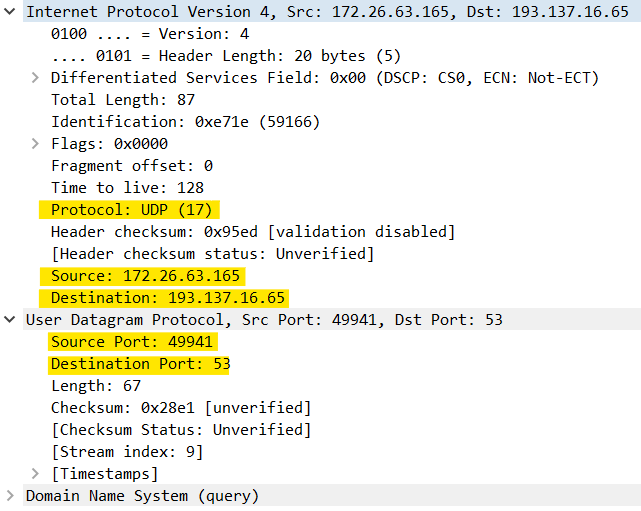
\includegraphics[scale=0.65]{PDU.png}
      \centering
      \caption{Exemplificação de PDU.}
      \label{fig:PDU}
      \end{figure}
  \end{enumerate}


  \begin{enumerate}[\textbf{b)}]
    \item \textbf{Utilizando o sniffer em modo de captura, proceda à invocação de várias aplicações conhecidas, nomeadamente:}
    \vspace{5mm}
    \begin{itemize}
        \item Acesso via browser ao URL: http://marco.uminho.pt
        \item Acesso ftp (anonymous): ftp.di.uminho.pt
        \item Acesso em tftp para router-ext (193.136.9.33)
        \item Acesso via telnet para router-ext (193.136.9.33) ou para\\*
        router-lab (192.168.90.254)
        \item Acesso ssh para qualquer host da sala de aula
        \item Resolução de nomes usando nslookup www.uminho.pt
        \item traceroute cisco.uminho.pt
    \end{itemize}
    \par \textbf{e construa uma tabela onde, para cada aplicação, conste o protocolo de transporte e a porta de atendimento do
    servidor (quando aplicável).}
    
    % Start new paragraph using alignment Justification 
    \vspace{5mm}
    
    \begin{table}[h!]
      \centering
      \begin{tabular}{p{4.4cm}  p{3cm}  p{3cm}} 
      \hline
      \textbf{Protocolo de Transporte} & \textbf{Porta de Origem} & \textbf{Porta de Destino}\\ [1ex] 
      \hline\hline
      HTTP & 53355 & 80 \\ [1ex]
      FTP & 20542 & 21 \\ [1ex]
      TFTP & 60499 & 69 \\ [1ex]
      TELNET & 545 & 23 \\ [1ex]
      SSH & 55608 & 22 \\ [1ex]
      DNS & 53068 & 53 \\ [1ex]
      ICMP & 53 & 55616 \\ [1ex] 
      \hline
      \end{tabular}
      \caption{Tabela de aplicações}
      \label{table:1}
      \end{table}


  \end{enumerate}

  % PART 2 START HERE!
  \section{Parte II - Filtragem de tráfego}

  \begin{enumerate}[\textbf{a)}]
    \item \textbf{Explore e descreva:}
    \begin{enumerate}[i]
      \item A utilidade dos filtros de captura e visualização;    
      \item A sintaxe e semântica dos filtros.
    \end{enumerate}
    \par\textbf{Dê alguns exemplos simples de utilização dos mesmos.}
    
    \begin{flushleft}
      \par Os filtros, tal como sugere, são opções que nos permitem selecionar um conjunto de informação a ser apresentadas no visualizador. Esse filtro pode ser utilizado por protocolo, endereço de rede, por porta, por endereço MAC.
      \par Eles possuem uma forma bem simples de se utilizar, basta aplicarmos no campo de pesquisa o que queremos mostrar. No exemplo a seguir iremos filtrar pelo protocolo TELNET.
      \begin{figure}[h]
        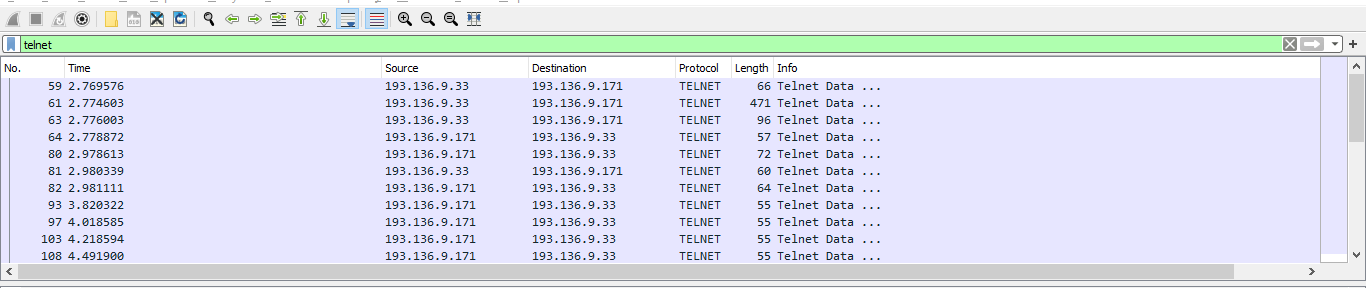
\includegraphics[scale=0.3]{filter01.png}
        \centering
        \caption{Exemplo aplicação do filtro TELNET.}
        \label{fig:filter01}
      \end{figure}
    \end{flushleft}
    
    \begin{flushleft}
      \par Como exemplo utilizamos o protocolo TELNET, e sua semântica de pesquisa, nesse caso, é bem simples, bastando apenas escrever o protocolo, mas caso queremos procurar o ip, a semântica permite adicionar outras informações, como o ip.dst, que seria o IP destino. 
      \begin{figure}[h]
        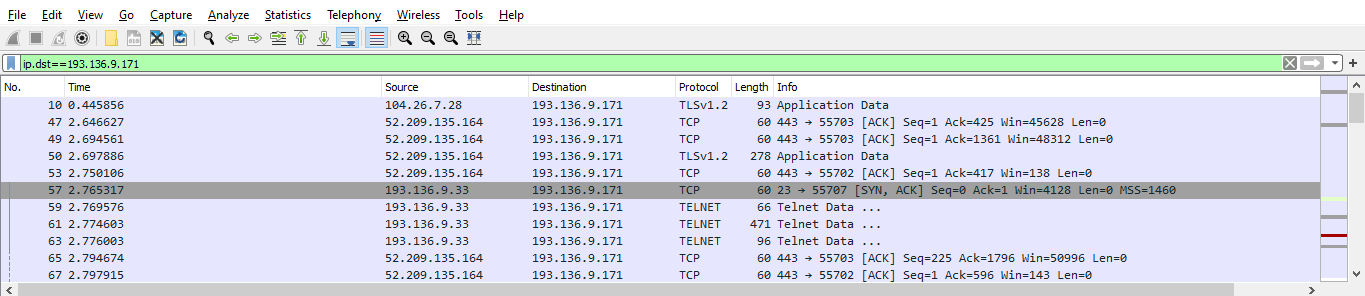
\includegraphics[scale=0.3]{filter02-dst.png}
        \centering
        \caption{Exemplo aplicação do filtro IP.DST.}
        \label{fig:filter02}
      \end{figure}
    \end{flushleft}

    \begin{flushleft}
      \par Também permite adicionar operadores lógicos, por exemplo o símbolo || que permite pesquisar dois protocolos ao mesmo tempo. 
      \begin{figure}[h]
        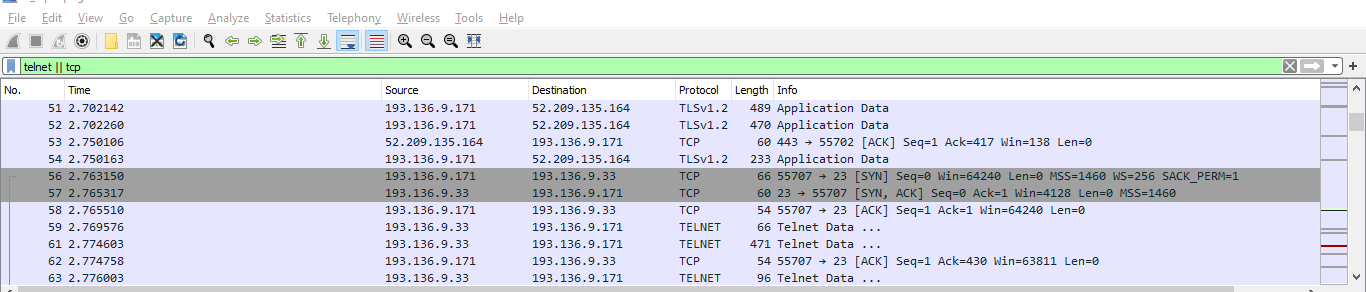
\includegraphics[scale=0.3]{filter03.png}
        \centering
        \caption{Exemplo aplicação do filtro com duplo parâmetros.}
        \label{fig:filter03}
      \end{figure}  
    \end{flushleft}

    \begin{flushleft}
      \par E por fim, o Wireshark possui uma opção no menu onde é possível consultar todos os filtros que existem para ser aplicado, e montar qual o filtro melhor se encaixa na pesquisa que deseja realizar. 
      \begin{figure}[h]
        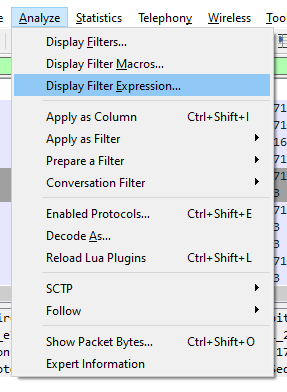
\includegraphics[scale=0.65]{menuwire01.png}
        \centering
        \caption{Aba para acesso ao menu avançado com todos os filtros.}
        \label{fig:menuwire01}
      \end{figure}  

      \begin{figure}[h]
        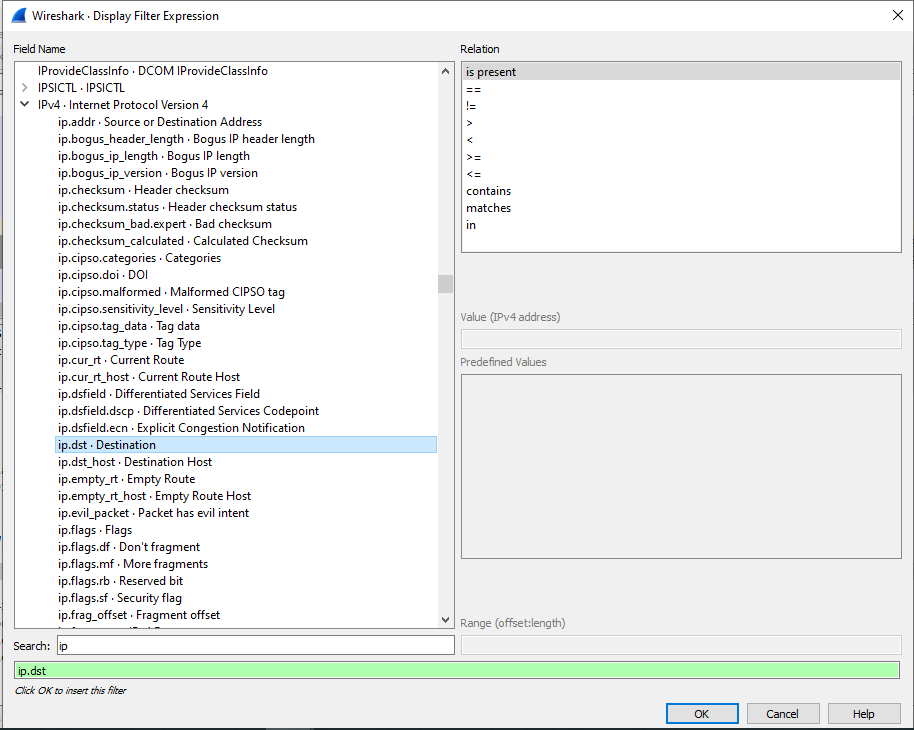
\includegraphics[scale=0.3]{menuwire02.png}
        \centering
        \caption{Display com todos os filtros.}
        \label{fig:menuwire02}
      \end{figure}  
    \end{flushleft}

  \end{enumerate}


  \begin{enumerate}[\textbf{b)}]
    \item  \textbf{Baseando-se nas tramas capturadas acima (1.b), e em outros exemplos que achar conveniente, explore a
    utilidade e utilização dos filtros de captura e visualização, nomeadamente na captura/visualização de:}
    \begin{itemize}
      \item protocolos aplicacionais;
      \item protocolos de transporte;
      \item endereços IP;
      \item pacotes com valores específicos nos campos principais dos cabeçalhos de transporte e rede (ver opção
      "+Expression");
      \item pacotes com flags de iniciação e termino de conexões TCP;
    \end{itemize}
    \par \textbf{Exemplifique a exploração que realizou, indicando a sintaxe utilizada nos filtros e, muito sucintamente os
    resultados obtidos.}
    
    \begin{flushleft}
      \par Aqui podemos mostrar a análise do arquivo gerado anteriormente. Em nosso exemplo vamos procurar a utilização de um protocolo para transferência de um ficheiro. Começamos por filtrar a captura, utilizando a sintaxe mais simples possível: TFTP. Podemos ver o resultado obtidos na imagem~\ref{fig:filtertftp}
      \begin{figure}[h]
        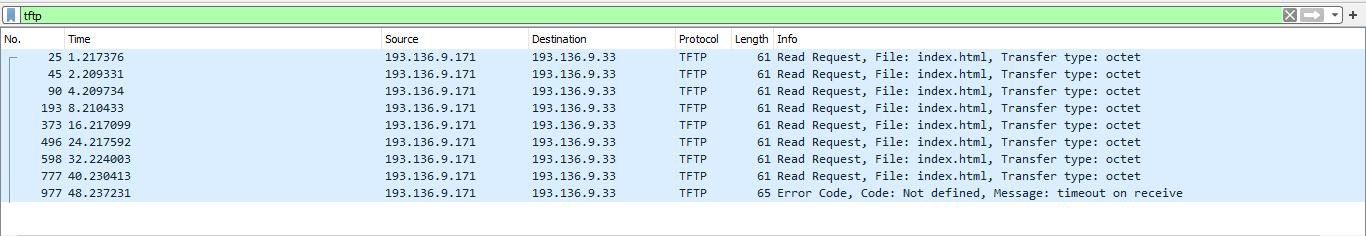
\includegraphics[scale=0.3]{filtertftp.png}
        \centering
        \caption{Aplicando o filtro para o protocolo TFTP.}
        \label{fig:filtertftp}
      \end{figure}  
    \end{flushleft}

    \begin{flushleft}
      \par Indo para a análise de um pacote, visualizando suas informações, podemos verificar que ele utiliza como protocolo de transporte o UDP (figura~\ref{fig:pdu01}), em seguida podemos verificar os endereços MAC dos dispositivos e os Ips utilizados (origem/Destino – figura~\ref{fig:pdu02}).
      \begin{figure}[h]
        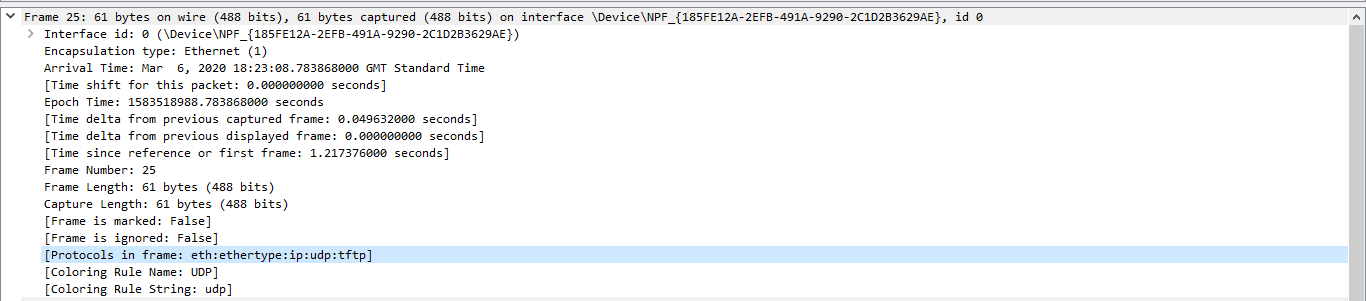
\includegraphics[scale=0.3]{pdu01.png}
        \centering
        \caption{Protocolo de transporte UDP.}
        \label{fig:pdu01}
      \end{figure} 

      \begin{figure}[h]
        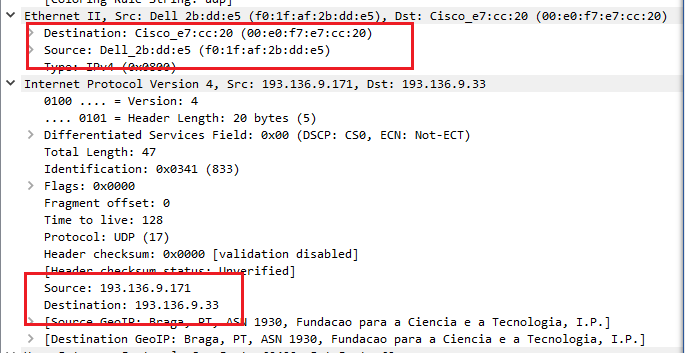
\includegraphics[scale=0.65]{pdu02.png}
        \centering
        \caption{Exibindo o MAC e IP dos hosts origem e destinos.}
        \label{fig:pdu02}
      \end{figure} 
    \end{flushleft}

    \begin{flushleft}
      \par E por último, nesse exemplo utilizado, podemos conferir as portas da aplicação que são utilizadas e como se trata de um protocolo com mensagem junto, ele nós informa qual o código enviado pela origem (figura~\ref{fig:pdu03}).
      \begin{figure}[h]
        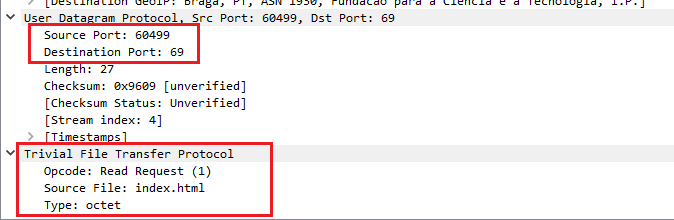
\includegraphics[scale=0.65]{pdu03.png}
        \centering
        \caption{Exibindo a porta de origem e destino para identificar a aplicação.}
        \label{fig:pdu03}
      \end{figure} 
    \end{flushleft}

    \begin{flushleft}
      \par E claro, ao montar o stream desse filtro(figura~\ref{fig:stream3}), podemos acompanhar qual foi a solicitação e a mensagem retornada pelo destino, conforme a figura~\ref{fig:followstream01}.
      \begin{figure}[h]
        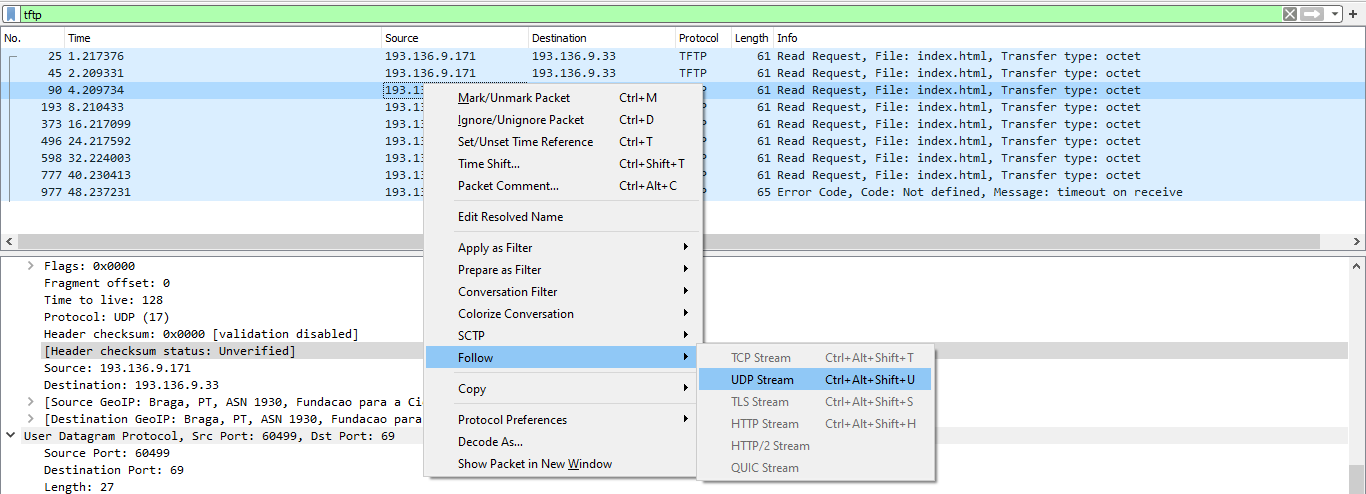
\includegraphics[scale=0.3]{stream3.png}
        \centering
        \caption{Menu para seguir o stream.}
        \label{fig:stream3}
      \end{figure} 
      \begin{figure}[h]
        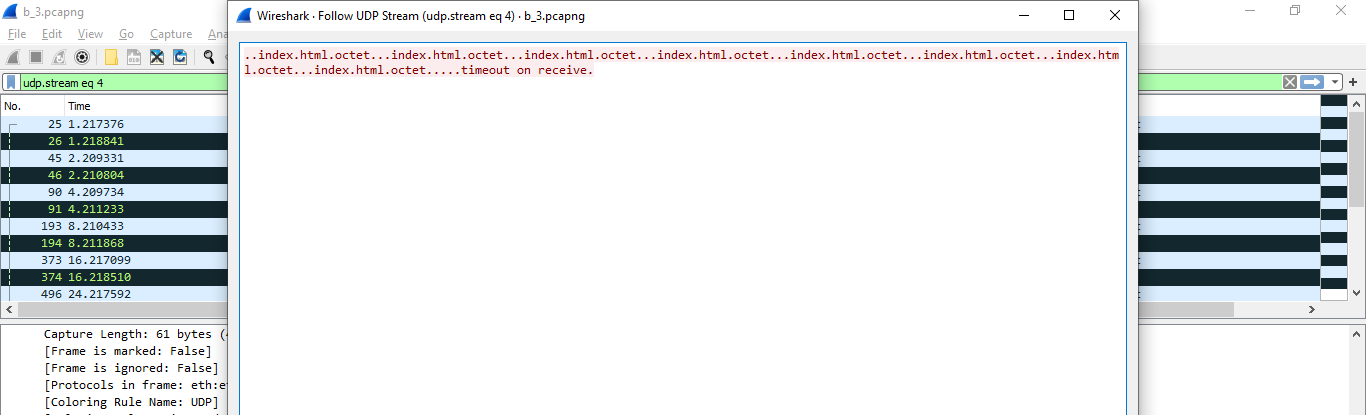
\includegraphics[scale=0.3]{followstream01.png}
        \centering
        \caption{Ao montar o stream, é apresentado as informações.}
        \label{fig:followstream01}
      \end{figure} 
    \end{flushleft}


  \end{enumerate}


  \begin{enumerate}[\textbf{c)}]
    \item \textbf{Para uma das aplicações que usam o protocolo TCP (e.g. Telnet router-ext), explore a opção "Analyse - Follow TCP Stream". Indique os filtros automaticamente aplicados por essa opção. Discuta eventuais fragilidades
    de segurança e confidencialidade dos dados.}
    
    \vspace{5mm}
    \begin{flushleft}
      \par Com a opção de filtragem via menu Analyse > Follow > TCP Stream, é possível selecionar um pacote entra vários capturados e reunir todos os pacotes que pertencem ao mesmo stream de dados. Neste caso foi feito inicialmente uma filtragem pelo protocolo Telnet, conforme visto na figura~\ref{fig:stream1} abaixo:
      \begin{figure}[h]
        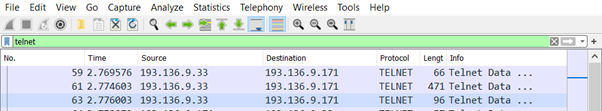
\includegraphics[scale=0.65]{stream1.png}
        \centering
        \caption{Exemplo lista de stream.}
        \label{fig:stream1}
      \end{figure}
    \end{flushleft}

    \begin{flushleft}
      \par Em seguida foi utilizado o menu Analyse > Follow > TCP Stream, mencionado anteriormente e com isso foi possível agrupar todos os pacotes pertencentes ao stream de pacotes pertencentes ao stream do pacote selecionado, inclusive aqueles que não são exclusivamente de protocolo Telnet, conforme visto a seguir na figura~\ref{fig:stream2}.
      \begin{figure}[h]
        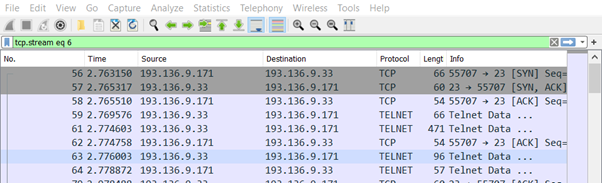
\includegraphics[scale=0.65]{stream2.png}
        \centering
        \caption{Exemplo lista de stream.}
        \label{fig:stream2}
      \end{figure}
    \end{flushleft}

    \begin{flushleft}
      \par Como pode também ser visto na figura~\ref{fig:stream2} o filtro que é gerado pelo menu executado basicamente é filtrar na captura pelo stream TCP de número 6 que sintaticamente possui a expressão (tcp.stream eq 6), o trecho tcp.stream indica intuitivamente que quer se filtrar por streams TCP e a parte (eq 6) indica que o stream especifico que se deseja é o de número igual (eq) a 6.
      \par E o mais interessante do resultado da ação executado pelo menu selecionado é a reconstrução e apresentação das trocas de mensagens trocadas entre origem e destino, de tal forma que seja possível capturar e entender uma troca de mensagens por completo, se forem enviados em texto claro, que é o caso do protocolo Telnet. Tal resultado é visualizado na figura~\ref{fig:followstream}
      \begin{figure}[h]
        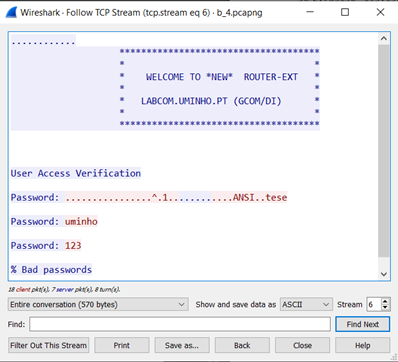
\includegraphics[scale=0.65]{followstream.png}
        \centering
        \caption{Montando o stream.}
        \label{fig:followstream}
      \end{figure}
    \end{flushleft}

    \begin{flushleft}
      \par Os trechos apresentados marcados em azul foram recebidos pelo destinatário e em vermelho pela a origem, que está a tentar aceder ao equipamento via protocolo Telnet. Assim vemos de forma clara o password que foi digitado pelo utilizador. Desta forma mostra a fragilidade do protocolo Telnet, bem como outros protocolos que transmitem suas mensagens via texto claro, caso sejam transmitidos conteúdos sensíveis como senhas, informações bancárias e outros, tais dados estarão expostos e a comprometer a confidencialidade das informações caso haja um utilizador malicioso a sniffar os pacotes que são transmitidos pela rede.
    \end{flushleft}
  \end{enumerate}


  \begin{enumerate}[\textbf{d)}]
    \item \textbf{Analise e identifique dados estatísticos da sua captura de pacotes.}

    \begin{flushleft}
      Dentre as capturas realizadas selecionou-se a referente ainda ao Telnet. Na tela principal já é possivel verificar a quantidade de pacotes capturados no total e quantos estão sendo exibidos, quando há um filtro aplicado.
      \par CRIAR TABELA AQUI:
      \par Quantidade de pacotes capturados: 352
      \par Total de pacotes exibidos: 50(14.2\%)
      \par Outra opção para se obter mais estatísticas é utilizar o menu Statistics, nele há uma lista de opções. Uma delas que é interessante é o Conversation, nesta são compiladas todas as conversas entre origm X e destindo Y para os protocolos Ethernet, Ipv4, Ipv6, TCP e UDP, sendo essas opções distribuídas em abas, conforme visto abaixo na figura~\ref{fig:conversation01}.
      \begin{figure}[h]
        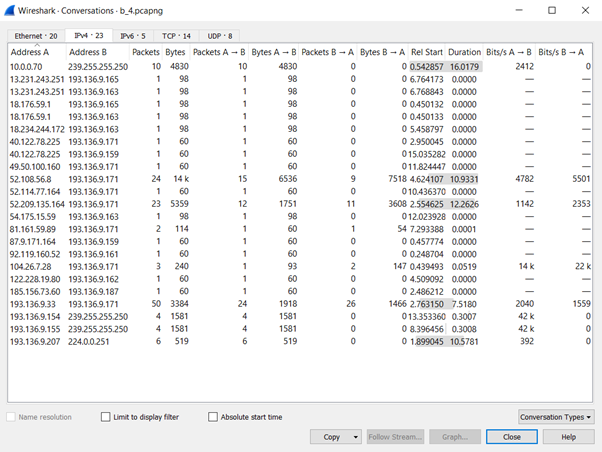
\includegraphics[scale=0.65]{conversation01.png}
        \centering
        \caption{Tabela conversation.}
        \label{fig:conversation01}
      \end{figure}
    \end{flushleft}

    \begin{flushleft}
      \par Outra estatistica interessante é listagem hierárquica dos protocolos, nela pode-se ver a representatividade de cada protocolo e subprotocolo no total da captura. Essa estatística pode ser visualizada na figura~\ref{fig:statistic}.
      \begin{figure}[h]
        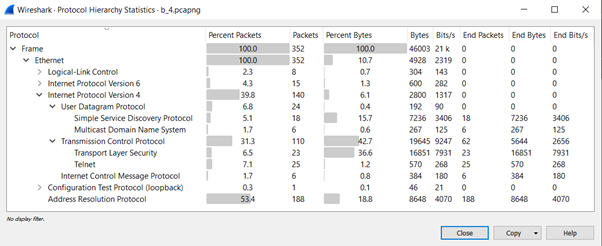
\includegraphics[scale=0.65]{statistic.png}
        \centering
        \caption{Tabela de estatística hierárquica.}
        \label{fig:statistic}
      \end{figure}
    \end{flushleft}

    \begin{flushleft}
      \par E outra forma de visualizar estatísticas é na opção File Properties do menu Statistics, que pode ser visualizado na figura~\ref{fig:details}
      \begin{figure}[h]
        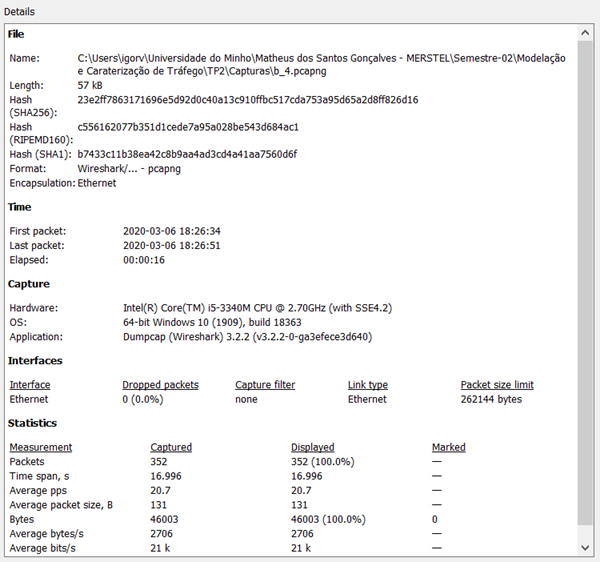
\includegraphics[scale=0.65]{details.png}
        \centering
        \caption{File Properties.}
        \label{fig:details}
      \end{figure}
      \par Quantidade de pacotes capturados: 352
      \par Total de pacotes exibidos: 50(14.2\%)
    \end{flushleft}

  \end{enumerate}

  \newpage

  \section{Conclusão}
    \begin{flushleft}
      Ao longo desse trabalho, tivemos a oportunidade de desenvolver nossas habilidades na análise do tráfego gerado.
      Com fácil aprendizado, a ferramenta Wireshark se mostra extremamente poderosa e eficaz, nos mostrando os detalhes das capturas geradas, com isso conseguimos caracterizar o tráfego, identificar as portas utilizadas e com isso qual o serviço utilizado, por exemplo.
      \par No relatório mostramos como podemos verificar tais informações, filtra os dados da captura, mostrando sua sintaxe e complexidade na geração dos filtro.
      Claro, estamos longe de sermos especialistas na caracterização e análise, mas podemos afirmar que estamos caminhando na direção correta.

    \end{flushleft}

\end{document}
